%%%%%%%%%%%%%%%%%%%%%%%%%%%%%%%%%%%%%%%%%%%%%%%%%%%%%%%%%%%%%%%%%%%%%%%%%%%%%%%%%%%%%
%                        Author: Harshit Prashant Dhanwalkar                        %
%%%%%%%%%%%%%%%%%%%%%%%%%%%%%%%%%%%%%%%%%%%%%%%%%%%%%%%%%%%%%%%%%%%%%%%%%%%%%%%%%%%%%

%-------------------------------------------------------------------------------------
%                    PACKAGES AND OTHER DOCUMENT CONFIGURATIONS                      %
%-------------------------------------------------------------------------------------

\documentclass[fleqn,10pt]{SelfArx} % Document font size and equations flushed left
\usepackage[english]{babel} 
\usepackage{enumitem}

\usepackage{tikz}
\usetikzlibrary{trees, positioning, shapes}
\usepackage{tikz-3dplot}
\tikzstyle{vertex}=[draw,fill=black!15,circle,minimum size=20pt,inner sep=0pt]
\tikzstyle{selected edge} = [draw,line width=5pt,-,red!50]

\usepackage{amsmath}
\usepackage{array} % for tables

\usepackage{pgfplots}
\pgfplotsset{compat=1.18}
\tdplotsetmaincoords{60}{115}
\pgfplotsset{compat=newest}

%-------------------------------------------------------------------------------------
%                                       COLUMNS                                      %
%-------------------------------------------------------------------------------------
\setlength{\columnsep}{0.55cm} % Distance between the two columns of text
\setlength{\fboxrule}{0.75pt} % Width of the border around the abstract

%-------------------------------------------------------------------------------------
%                                        COLORS                                      %
%-------------------------------------------------------------------------------------
\definecolor{color1}{RGB}{0,0,90} % Color of the article title and sections
\definecolor{color2}{RGB}{0,20,20} % Color of the boxes behind the abstract and headings

%-------------------------------------------------------------------------------------
%                                       EQUATIONS                                    %
%-------------------------------------------------------------------------------------
\usepackage{cancel} % for crossing the word showing it is cancelled or is zero

%-------------------------------------------------------------------------------------
%                                     EQUATIONLINKS                                  %
%-------------------------------------------------------------------------------------
\newcommand{\myeqref}[1]{\textcolor{blue}{\textup{(\getrefnumber{#1})}}}

%-------------------------------------------------------------------------------------
%                                       HYPERLINKS                                   %
%-------------------------------------------------------------------------------------
\usepackage{xcolor}
\usepackage{hyperref}
\usepackage{footnote}

%\newcommand{\myhref}[2]{\href{#1}{\textcolor{blue}{#2}}}
\newcommand{\myhref}[2]{%
  \href{#1}{\textcolor{blue}{#2}}%
  \footnote{\url{#1}}%
}

\usepackage{cleveref}
% Customize cleveref to use "Eq." for equations
\crefname{equation}{Eq.}{Eq.}
\Crefname{equation}{Eq.}{Eq.}

\hypersetup{
	hidelinks,
	colorlinks,
	breaklinks=true,
	urlcolor=color2,
	citecolor=color1,
	linkcolor=color1,
	bookmarksopen=false,
	pdftitle={Title},
	pdfauthor={Author},
}

% ------------------------------------------------------------------------------------
%                                       CUSTOM  SYMBOLS                              %
%-------------------------------------------------------------------------------------
\newcommand{\zbar}{\raisebox{0.2ex}{--}\kern-0.6em Z}

%-------------------------------------------------------------------------------------
%                                       ARTICLE INFORMATION                          %
%-------------------------------------------------------------------------------------
\JournalInfo{Dual Degree Engineering Physics, 8$^{th}$ Semester, 2024} % Journal information
\Archive{Mtech, Earth System Sciences (ESS), 1$^{st}$ year} % Additional notes (e.g. copyright, DOI, review/research article)

\PaperTitle{Lecture Notes on Boundary Layer Meteorology} % Article title

\Authors{Harshit Prashant Dhanwalkar (SC21B164)\textsuperscript{1}*} % Authors
\affiliation{\textsuperscript{1}\textit{MTech, Earth System Sciences (ESS), 1$^{st}$ year, Department of Physics, Indian Institute Of Spacescience and Technology (IIST)}} % Author affiliation
\affiliation{*\textbf{email}: harshitpd1729@gamil.com} % Corresponding author

\Keywords{} % Keywords - if you don't want any simply remove all the text between the curly brackets
\newcommand{\keywordname}{Keywords} % Defines the keywords heading name

%-------------------------------------------------------------------------------------
%                                           ABSTRACT                                 %
%-------------------------------------------------------------------------------------
\Abstract{Notes of Lectures and addional information from books.}

%-------------------------------------------------------------------------------------
%                                            DOCUMENT                                %
%-------------------------------------------------------------------------------------
\begin{document}
\maketitle % Output the title and abstract box
\clearpage
\tableofcontents % Output the contents section
\clearpage
\thispagestyle{empty} % Removes page numbering from the first page
\clearpage

%-------------------------------------------------------------------------------------
%                                       DOCUMENT CONTENTS                           %
%-------------------------------------------------------------------------------------
%\addcontentsline{toc}{section}{Introduction} % Adds this section to the table of contents
%-------------------------------------------------------------------------------------
\section{Lecture 1 09/01/2025}
\subsection{Introduction to Boundary Layer}
The Boundary Layer can be defined as part of  the troposphere that is directly influenced by the presence of the Earth's surface and responds to surface forcings with a time scale of about an hour or less.

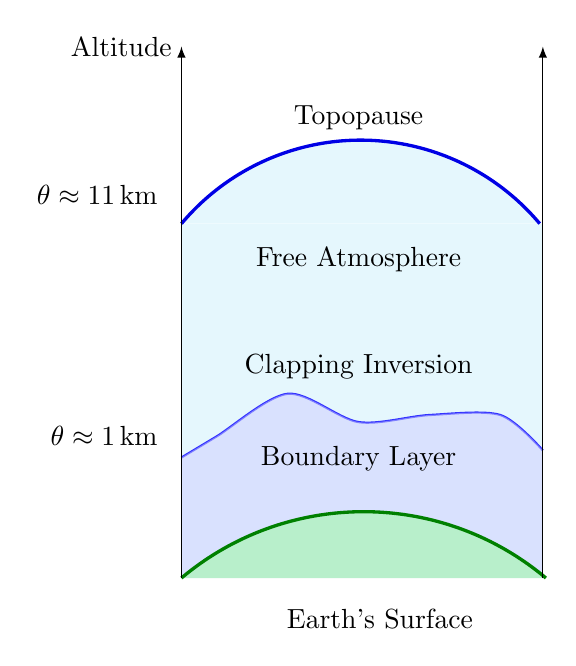
\begin{tikzpicture}[scale=0.9]
	%Free Atmosphere curve
	\fill[cyan!20, opacity=0.5] (-0.5,0) rectangle (4.6,5);
	\fill[cyan!20, opacity=0.5]
	(-0.5,5) arc[start angle=140, end angle=40, radius=3.3cm] -- (4.6,5) -- cycle;
	\draw[very thick, blue!90!black]
	(-0.5,5) arc[start angle=140, end angle=40, radius=3.3cm];
	\node[anchor=north] at (2,4.8) {Free Atmosphere};
	%Topopause curve
	\node[anchor=north] at (2,6.8) {Topopause};
	%Clapping Inversion curve
	\draw[thick,blue!80] plot [smooth] coordinates {(-0.5, 1.7) (0,2) (1,2.6) (2,2.2) (3,2.3) (4,2.3) (4.6,1.8)};
	\fill[blue!20,opacity=0.5] (-0.5,0) -- plot [smooth] coordinates {(-0.5, 1.7) (0,2) (1,2.6) (2,2.2) (3,2.3) (4,2.3) (4.6,1.8)}  -- (4.6,0) -- cycle;
	\node[anchor=north] at (2,3.3) {Clapping Inversion};
	% Boundary layer curve
	\node[anchor=north] at (2,2) {Boundary Layer};
	% Earth's surface
	\fill[green!40,opacity=0.5]
	(2.5-3,0) arc[start angle=130, end angle=50, radius=4cm] -- (2.5,0) -- cycle;
	\draw[very thick, green!50!black, shift={(2.5,0)}]
	(-3,0) arc[start angle=130, end angle=50, radius=4cm];
	\node[anchor=north] at (2.3,-0.3) {Earth's Surface};
	% Axis label
	\draw[-latex] (-0.5,0) -- (-0.5,7.5) node[anchor=east] {Altitude};
	\draw[-latex] (4.6,0) -- (4.6,7.5) node[anchor=east] {};
	% Labels
	\node[anchor=east] at (-0.7,5.4) {\(\theta \approx 11 \, \mathrm{km}\)};
	\node[anchor=east] at (-0.7,2) {\(\theta \approx 1 \, \mathrm{km}\)};
\end{tikzpicture}

\subsection{Boundary layer forcing mecchanism}
What physical process modify boundary layer air parcel?
\begin{enumerate}[noitemsep]
	\item Heat transfer to.from the ground.
	\item Frictional drag.
	\item Evaporation/transpiration.
	\item Terrain-induced flow modification.
	\item Pollution emission.
\end{enumerate}

\subsection{Types of air flow or wind}
Air flow or wind can be decomposed into following 3 types:
\begin{enumerate}[noitemsep]
	\item Mean wind
	\item Turbulence
	\item Waves
\end{enumerate}
\end{document}
